\subsection{Architektur}

Die Grundstruktur des Programms folgt dem Prinzip der \glslink{Model-View-Controller}{MVC}-Architektur. Die Unterteilung der Submodule in Model, View und Controller ermöglicht eine leichte Modifikation und Erweiterung.

\begin{figure}[H]
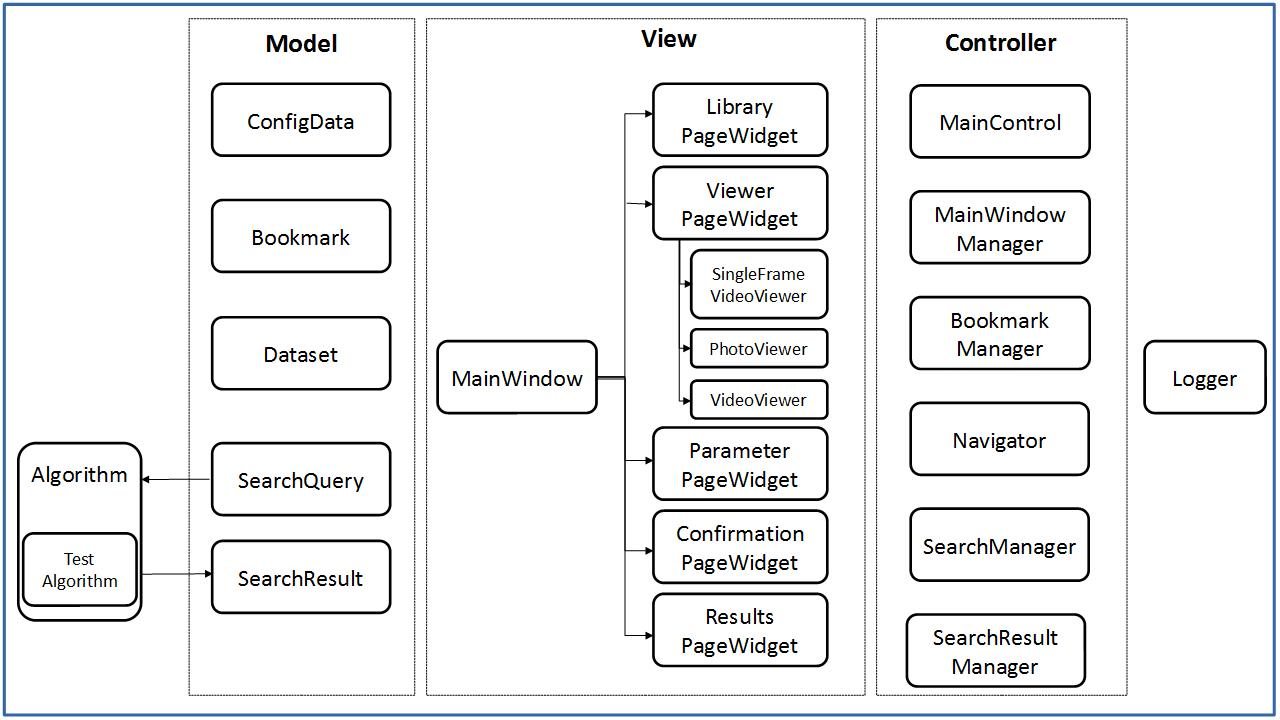
\includegraphics[width=1\linewidth]{img/architektur}
\caption{Architektur}
\label{fig:architektur}
\end{figure}

\begin{itemize}
\item \glslink{Suchalgorithmus}{Algorithm}\newline
Verschiedene austauschbare inhaltsbasierte \glslink{Suchalgorithmus}{Suchalgorithmen}. Die Algorithmen verwenden die Klassen des Models, ausgenommen ConfigData und die Klassen, die zur Verwaltung von Bookmarks gehören. 
\item TestAlgorithm\newline
Ein \gls{Suchalgorithmus}, der zu Testzwecken implementiert wird.
\item Logger \newline
Der Logger dokumentiert den Verlauf des Programms (Aktivitäten, Suchlaufzeit, Fehlermeldungen, ...). Das Protokoll wird z.B. in einer Log-Datei gespeichert. Prinzipiell ist die Log-Datei nur für Entwickler interessant. Der Benutzer kann jedoch diese Datei mitansehen, in dem er das Programm mit speziellen Argumenten startet.
\end{itemize}

\subsection*{Model}
\begin{itemize}
\item ConfigData \newline
Die Konfigurationsdaten passen die Anwendung an die Präferenzen des Benutzers an: Die gewählte Sprache und die Aktivierung bzw. Deaktivierung des Benachrichtigungstons werden gespeichert und beim erneuten Starten der Anwendung als Voreinstellung gesetzt. Außerdem wird eine Hilfe-Datei gespeichert.
\item Bookmark \newline
Suchergebnisse werden in der Chronik oder als Bookmark gespeichert.
\item Dataset \newline
Die Bilder und Videos bilden eine Grundlage der Anwendung, außerdem kann ein Datensatz \glslink{Annotation} {Annotationen} enthalten.
\item SearchQuery \newline
Die Suchanfrage ist der Input für das Verfahren. CoBaB generiert eine Suchanfrage, die aus gewählter Suchvorlage, gewünschtem \gls{Suchalgorithmus}, den Suchparametern und dem Suchraum besteht. Der Suchraum ist durch die Datensätze festgelegt, in denen gesucht werden soll.
\item SearchResult \newline
Der \gls{Suchalgorithmus} generiert ein Suchergebnis.
\end{itemize}

\subsection*{View}
\begin{itemize}
\item MainWindow \newline
Das MainWindow ist das Hauptfenster von CoBaB. Es zeigt die Widgets an.

\item LibraryPageWidget \newline
Die Bibliothek ist beim Starten des Programms zu sehen. Anfangs ist nur eine voreingestellte Auswahl an Datensätzen zu sehen. Jedes Mal beim erneuten Öffnen werden die zuletzt genutzten Datensätze angezeigt. Man kann entweder einen Datensatz aus den angezeigten wählen oder über einen Auswahl-Dialog einen neuen suchen.

\item ViewerPageWidget \newline
Nach der Auswahl eines Datensatzes, wird der Inhalt angezeigt. Dem Datensatz entsprechend wird der SingleFrameVideoViewer, PhotoViewer oder der VideoViewer integriert, um dem Benuter den Datensatz grafisch anzuzeigen und die Wahl einer Vorlage zu ermöglichen.

\item ParameterPageWidget \newline
Die \glslink{Suchalgorithmus}{Suchalgorithmen} stellen eine Parameterdatei bereit. In diesem Widget können die Parameter eingestellt werden.

\item ConfirmationPageWidget \newline 
Dieses Widget zeigt die Zusammenstellung der gewünschten Auswahl an.

\item ResultsPageWidget \newline
Die Ergebnisse der Suche werden in diesem Widget angezeigt. Die Suchergebnisse (Bilder/Videos) werden von meist zutreffend zu weniger zutreffend aufgelistet. 

\end{itemize}
\subsection*{Controller}
\begin{itemize}
\item MainControl \newline
Steuert den korrekten Ablauf von CoBaB.

\item MainWindowManager \newline
Der MainWindowManager stellt die Bookmarks und Chronikeinträge dem MainWindow zur Verfügung.

\item BookmarkManager \newline
Der BookmarkManager ist für die Verwaltung der Bookmarks und Chronikeinträge zuständig.

\item Navigator \newline
Der Navigator ist in der Lage, die PageWidgets zu wechseln. Des weiteren ist er für den Austausch von Daten zwischen den PageWidgets verantwortlich.

\item SearchManager \newline
Dieser Manager startet oder beendet eine Suchanfrage.

\item SearchResultManager \newline
Diese Komponente sammelt die Suchergebnisse (Bewertung der Bilder/Videos durch den Algorithmus) und sortiert diese absteigend.
\end{itemize}
\pagebreak


\subsection{Klassendiagramm}

Das folgende Diagramm zeigt eine Übersicht aller Klassen.

\begin{figure}[H]
	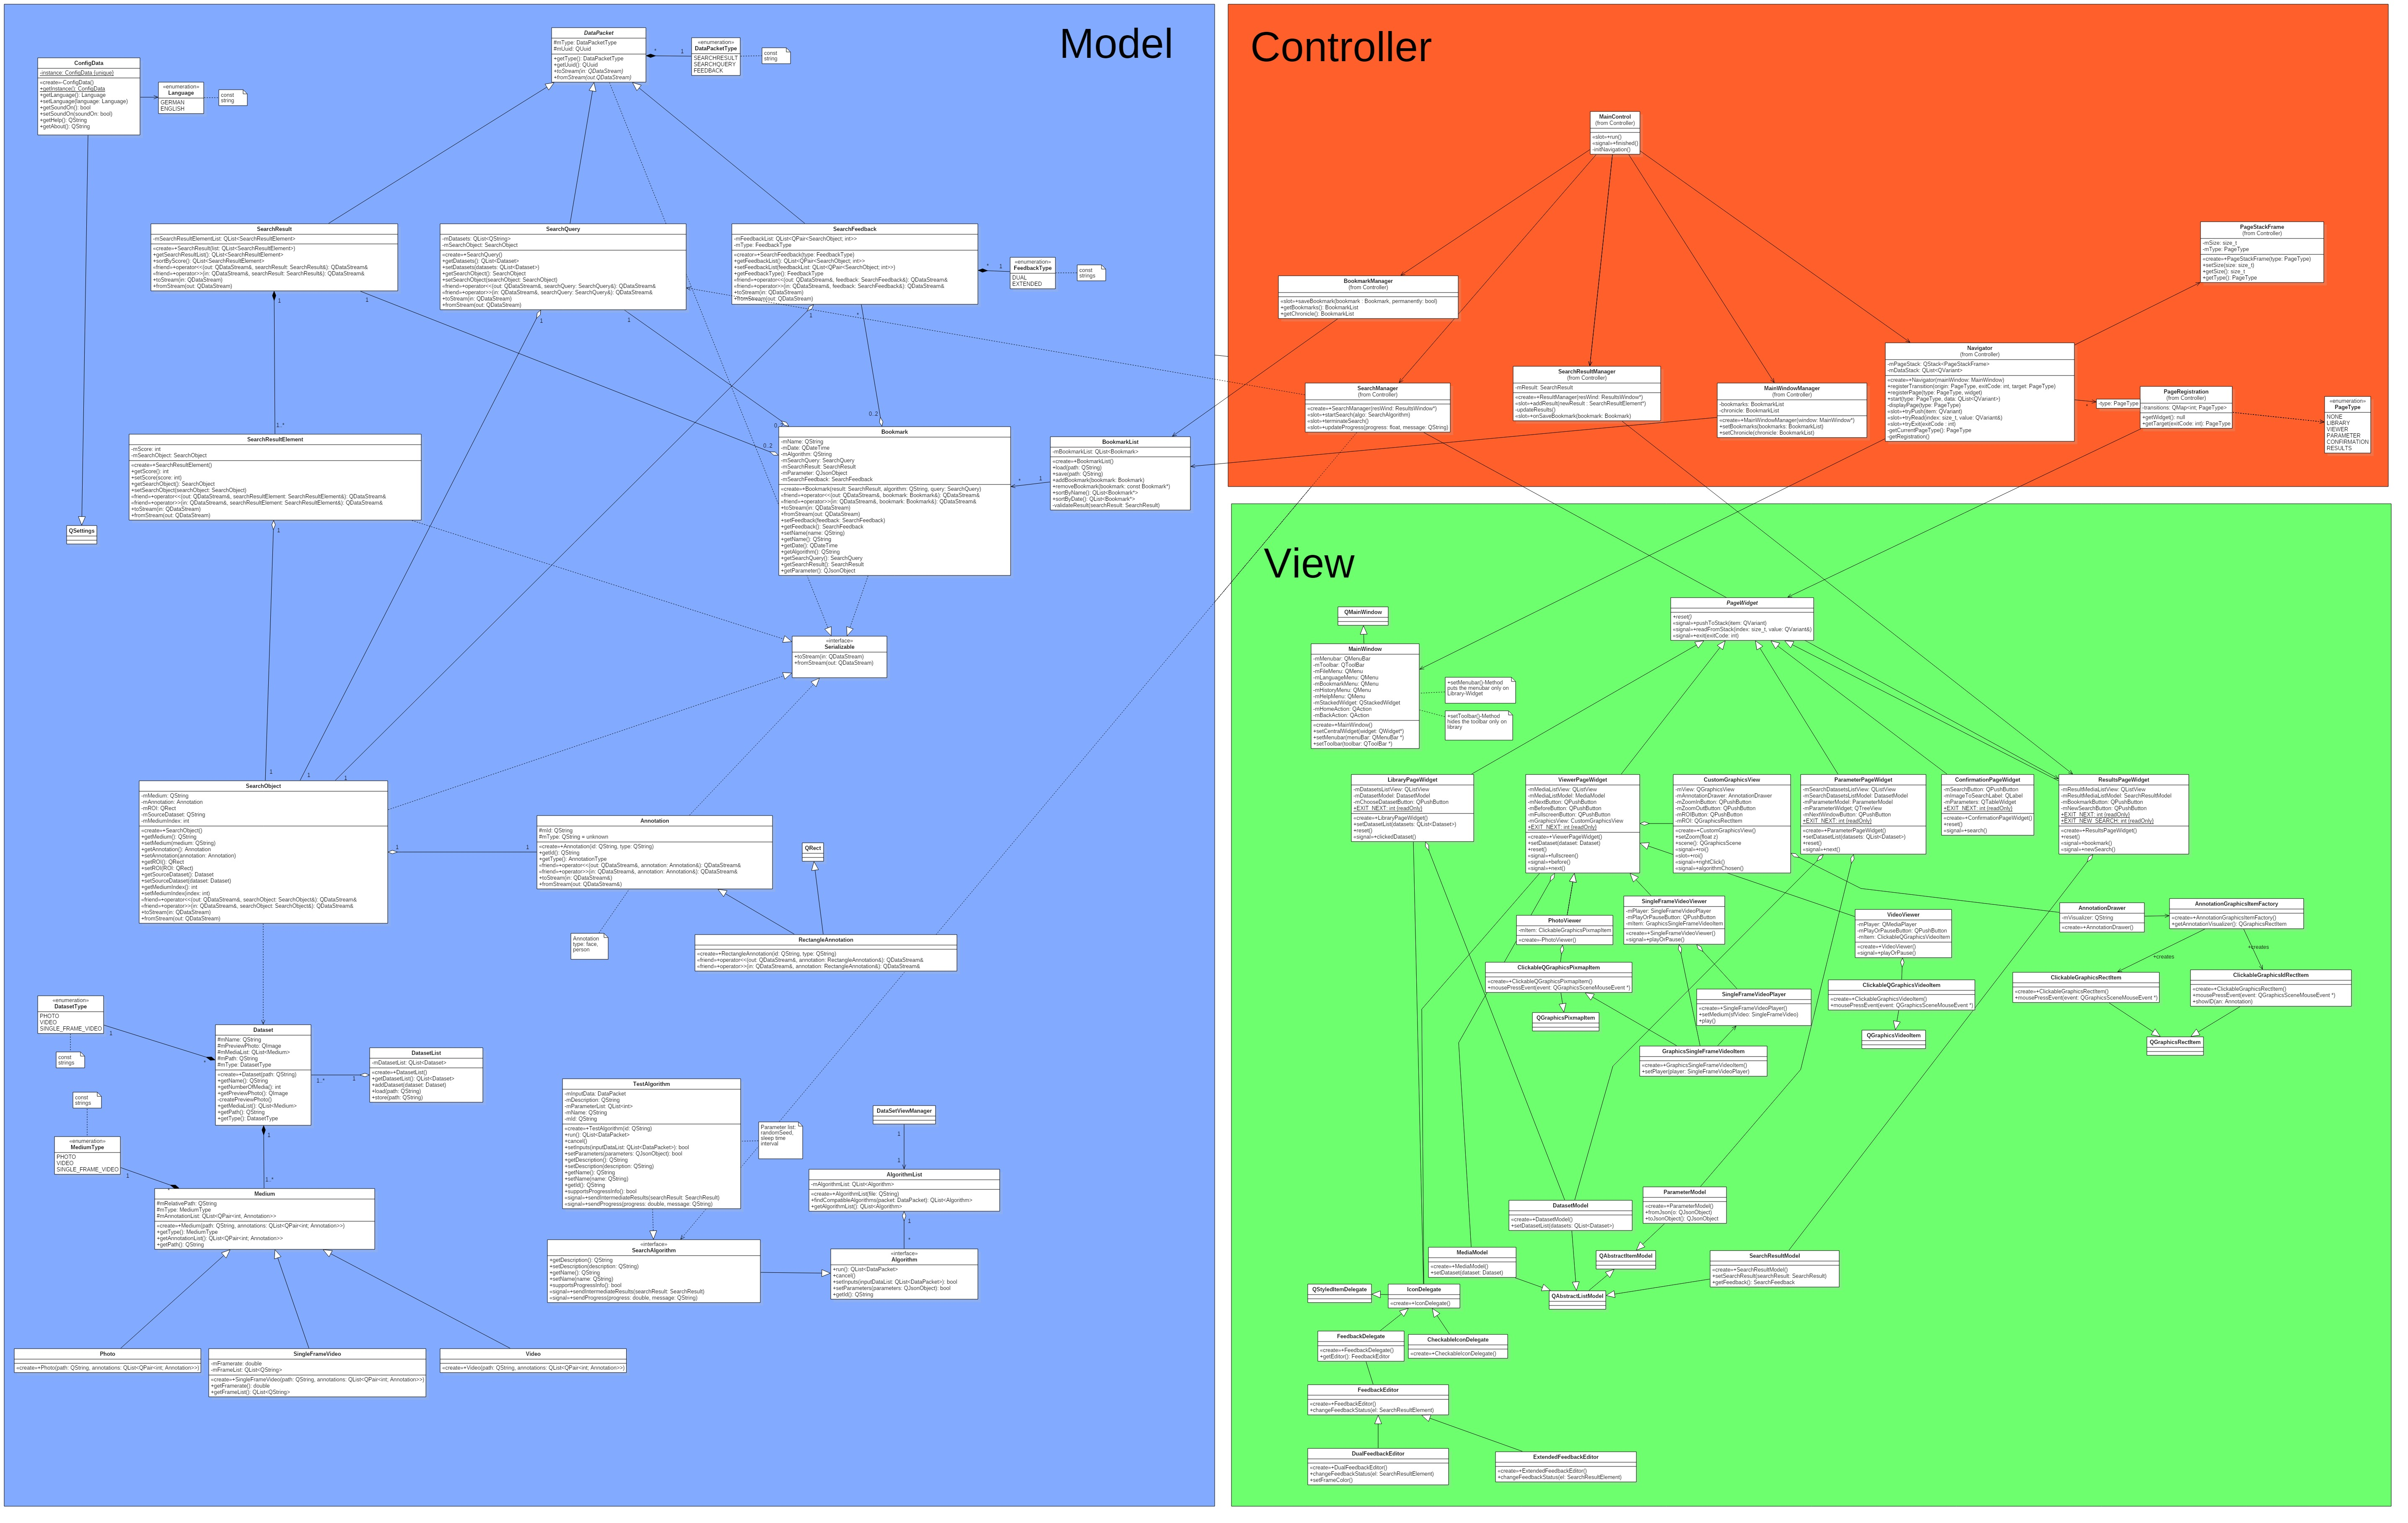
\includegraphics[width=1\linewidth]{img/Klassendiagramm/Complete}
	\caption{Klassendiagramm}
	\label{fig:klassendiagramm}
\end{figure}

